

\chapter{System Design}

This chapter outlines the chosen methodology for the UAV navigation system, detailing the pipeline and its various components. The system is designed to accurately estimate the UAV's position and heading, even in scenarios where GPS data is unreliable or unavailable. The high-level flow of the system is illustrated in Figure \ref{fig:HighLevelFlow}.

\begin{figure}[H]
    \centering
    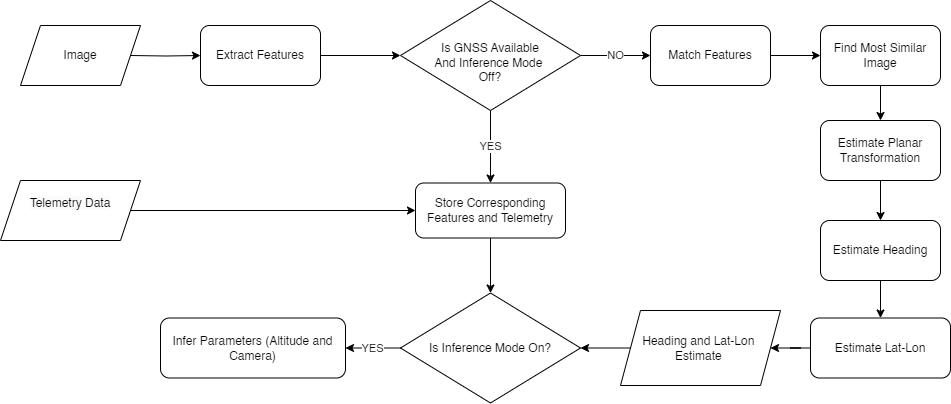
\includegraphics[width=0.8\textwidth]{Chapter 3/Chap3Figs/HighLevelFlow.png}
    \caption{High-Level Flow of the System}
    \label{fig:HighLevelFlow}
\end{figure}




\section{System Pipeline}

The UAV image-processing pipeline comprises several stages, each addressing specific goals in the larger aim to estimate the new GPS and heading of the UAV. These stages require varying levels of precision and efficiency to ensure robust performance.

\subsection{Pipeline Stages}

\begin{enumerate}
    \item \textbf{Image Input:}  
    The process begins with capturing a live image from the UAV’s downward-facing camera. This real-time visual input provides essential information about the UAV’s environment, forming the basis for position estimation.

    \item \textbf{Feature Extraction:}  
    Keypoints and descriptors are extracted from the current image to aid in the matching process. This extraction occurs in two layers:
    \begin{enumerate}
        \item \textbf{Coarse Layer:} Used for proximity search space reduction.
        \item \textbf{Dense Layer:} Used for precise matching and transformation estimation. 
    \end{enumerate}
    By also performing feature extraction when GPS is available, the system reduces computational load during the critical phase when GPS is lost. 

    \item \textbf{Storage (Telemetry and Features):}  
    Extracted features (keypoints and descriptors) along with telemetry data (GPS position and heading) are stored for future reference. Stored features facilitate relative transformation inference when GPS is unavailable, while telemetry data assists in converting relative transformations to real-world coordinates and headings.

    \item \textbf{Match Features:}  
    Features between the current image and reference images are matched to ensure that comparisons are based on mutual features. This involves two matching stages:
    \begin{enumerate}
        \item \textbf{Coarse Matching:} Matches the coarse layer of features to reduce the search space.
        \item \textbf{Dense Matching:} Matches the dense layer for precise position estimation.
    \end{enumerate}
    The matching process is optimized to ensure robustness against noise and outliers, with a focus on computational efficiency. The techniques are as follows:
    \begin{enumerate}
        \item \textbf{Feature Matching:}  
        Utilizes FLANN and BruteForce matchers to identify potential matches between the current and reference images. The matchers are optimized to ensure robustness against noise and outliers, with a focus on computational efficiency.
        
        \item \textbf{Optimization:}  
        Refines the matches using techniques such as Lowe's ratio test, n-Match thresholding, and absolute thresholding to ensure that only high-quality matches are considered for further processing. This refinement step is crucial for accurate transformation estimation. 

    \item \textbf{Similarity Comparison:}  
    The system compares the input image with reference images to identify the most similar one. This comparison is conducted using global matching techniques on aligned images to ensure efficiency and accuracy.
    \begin{enumerate}
        \item \textbf{Proximity Search Space Reduction:}  
        Reduces the search space based on proximity from the last known or estimated GPS location. A fixed radius was initially used, but later updated to return a specific number of the closest matches. 
        
        \item \textbf{Rotational Alignment:}  
        Estimates the rotation between the input and reference images using the coarse layer of features. The images are aligned using the course estimate as global matchers tolerate minor rotational inaccuracies well.
        
        \item \textbf{Best Match Identification:}  
        Computes similarity scores between the input image and each candidate image using global matching techniques. The image with the highest similarity score is selected as the best match, serving as the reference for position estimation.
    \end{enumerate}



    \item \textbf{Planar Transformation Estimation:}  
    After identifying the best match, the system performs a precise estimation of both rotation and translation between the input and reference images using the dense match layer. This involves several sub-steps to enhance accuracy:
    \begin{enumerate}
        \item \textbf{Angle Estimation:}  
        Utilizes the chosen transformation method to obtain a precise estimate of the rotation between the input and reference images, forming the basis for heading estimation.
        
        \item \textbf{Image Alignment \& Recomputation of Dense Layer:}  
        Aligns the input image with the reference image based on the estimated rotation, thereby implicitly removing non-mutual information by rotating it off the canvas. The dense layer of features is recomputed on the aligned images to ensure accurate translation estimates.
        
        \item \textbf{Translation Estimate:}  
        Performs a precise estimation of translation between the two images using the refined dense layer, providing the basis for GPS inference.
    \end{enumerate}

    \item \textbf{Update to Global Coordinate System:}  
    The estimated translation, initially in the internal image coordinate system (pixels), must be converted to real-world coordinates (metres) and then to the global coordinate system (longitude and latitude). This conversion involves several stages:
    \begin{enumerate}
        \item \textbf{Heading Update:}  
        Adds the estimated rotation to the reference image's heading to determine the UAV's new heading.
        
        \item \textbf{Translation Rotation from Internal to Global Coordinate System:}  
        Rotates the translation vector by the UAV's estimated global heading to align it with the global coordinate system without altering its magnitude.
        
        \item \textbf{Pixel to Metres (Relative):}  
        Converts the estimated change in pixels to metres using the dynamically inferred conversion factor. 
        
        \item \textbf{Metres to Global Coordinate System (Relative):}  
        Translates the metre-based changes to relative changes in longitude and latitude using the following equations:
        \begin{equation}
            \Delta \text{Longitude} = \frac{\Delta \text{Metres}}{111320 \times \cos(\text{Latitude})}
        \end{equation}
        \begin{equation}
            \Delta \text{Latitude} = \frac{\Delta \text{Metres}}{111320}
        \end{equation}
        These calculations account for the Earth's oblate spheroid shape, ensuring accurate positional data by adjusting for the decreasing distance between longitudes as one moves towards the poles.
        
        \item \textbf{Conversion to Absolute GPS:}  
        Adds the relative changes in longitude and latitude to the GPS coordinates of the reference image, resulting in the UAV's new GPS position.
    \end{enumerate}

    \item \textbf{Output New GPS and Heading:}  
    The calculated translation and rotation values are used to estimate the UAV's new GPS coordinates and heading. This enables pilots to navigate the UAV back to its base along the original path, even in the absence of GPS.

    \item \textbf{Dynamic Parameter Inference:}  
    This stage is performed while GPS is available. It estimates the GPS position using a temporary pixel-to-metre conversion factor of 1, utilizing the pipeline's stages to compute this estimate. The estimated GPS is compared to the ground truth GPS, and the difference is used to adjust the pixel-to-metre conversion factor. This ensures accurate conversion across datasets with varying altitudes. The first five images are used to infer this scaling factor.


\end{enumerate}


\section*{Dynamic Methods and Techniques}
Upon rigorous testing, it was seen that many parameters in the pipeline simply cannot generalize without tuning. This included the parameters of some feature detectors, optimization techniques, and search space reduction methods. To address this, dynamic methods were implemented to adjust these parameters based on the current scenario. The following dynamic methods were implemented:

% begin itemize
\begin{itemize}
    \item \textbf{Dynamic Feature Detector Selection:} AKAZE, the only detector without a dedicated keypoint target parameter (such as ORB's nFeatures), was highly accurate when tuned. However, the leniency threshold of AKAZE was found to be inconsistent across datasets. To address this, a dynamic method was implemented to adjust the leniency threshold based on the number of keypoints detected. This ensures that the detector is neither too lenient nor too strict, providing a balance between accuracy and efficiency.
    \item \textbf{Lowe's Ratio:} Lowe's ratio test is a critical step in the matching process, ensuring that only high-quality matches are considered for further processing. However, the optimal threshold for this test varies highly across datasets and scenarios. To address this, a dynamic method was implemented to adjust the Lowe's ratio threshold, starting at a strict threshold, and gradually relaxing it until a sufficient number of matches are found. This ensures that the system remains robust against noise and outliers while maintaining computational efficiency.
\end{itemize}

The above dynamic methods ensure that the system remains stable in different scenarios, adapting to varying conditions to provide accurate and efficient performance. However, these methods still, in part, fail to understand the nuances of the dataset perfectly. In the future, in flight error to ground truth estimates can be used to iteratively solve for the most optimal static parameters for the given environment, assuming it does not significantly change during flight. Alternatively, a dedicated machine learning model can be trained to predict and constantly adjust the optimal parameters based on the dataset's characteristics in-flight, providing a more robust and efficient solution.


\section*{Rotational Normalization Strategies}

Rotational normalization is essential for aligning images and translating estimations accurately in image-based UAV navigation systems. Two primary strategies were considered for normalizing rotations during the flight back to the base. The first involves applying rotational normalization during image capture, which aligns both images to a global North-East (NE) reference space before keypoint detection. The second method avoids normalization at the point of capture, aligning the images relative to one another and applying normalization only after translation estimation.

The key difference between these two methods lies in their respective losses caused by image rotation, due to the fixed canvas size during normalization. When an image is rotated, parts of the image are lost or moved off-canvas. 
The loss function for the first approach, where images are normalized independently, is proportional to:

\begin{equation}
\text{Loss}_{\text{pre}} \propto |\sin(|\Delta_1|) + \sin(|\Delta_2|)|
\end{equation}

In the second approach, where images are aligned relative to each other before normalization is applied, the loss function is:

\begin{equation}
\text{Loss}_{\text{post}} \propto |\sin(|\Delta_2 - \Delta_1|)|
\end{equation}


Here, the loss depends on the relative difference in rotation between the two images, reducing the potential for compounded information loss. In the given application, during the return flight to base, the UAV will undergo an initial 180-degree rotation relative to the outbound path with an expected maximum tolerance of ±20 degrees as the UAV attempts to as accurately as possible follow the path back to base. Given this constraint, the loss functions of both approaches are proportional to the following diagram:

\begin{figure}[H]
    \centering
    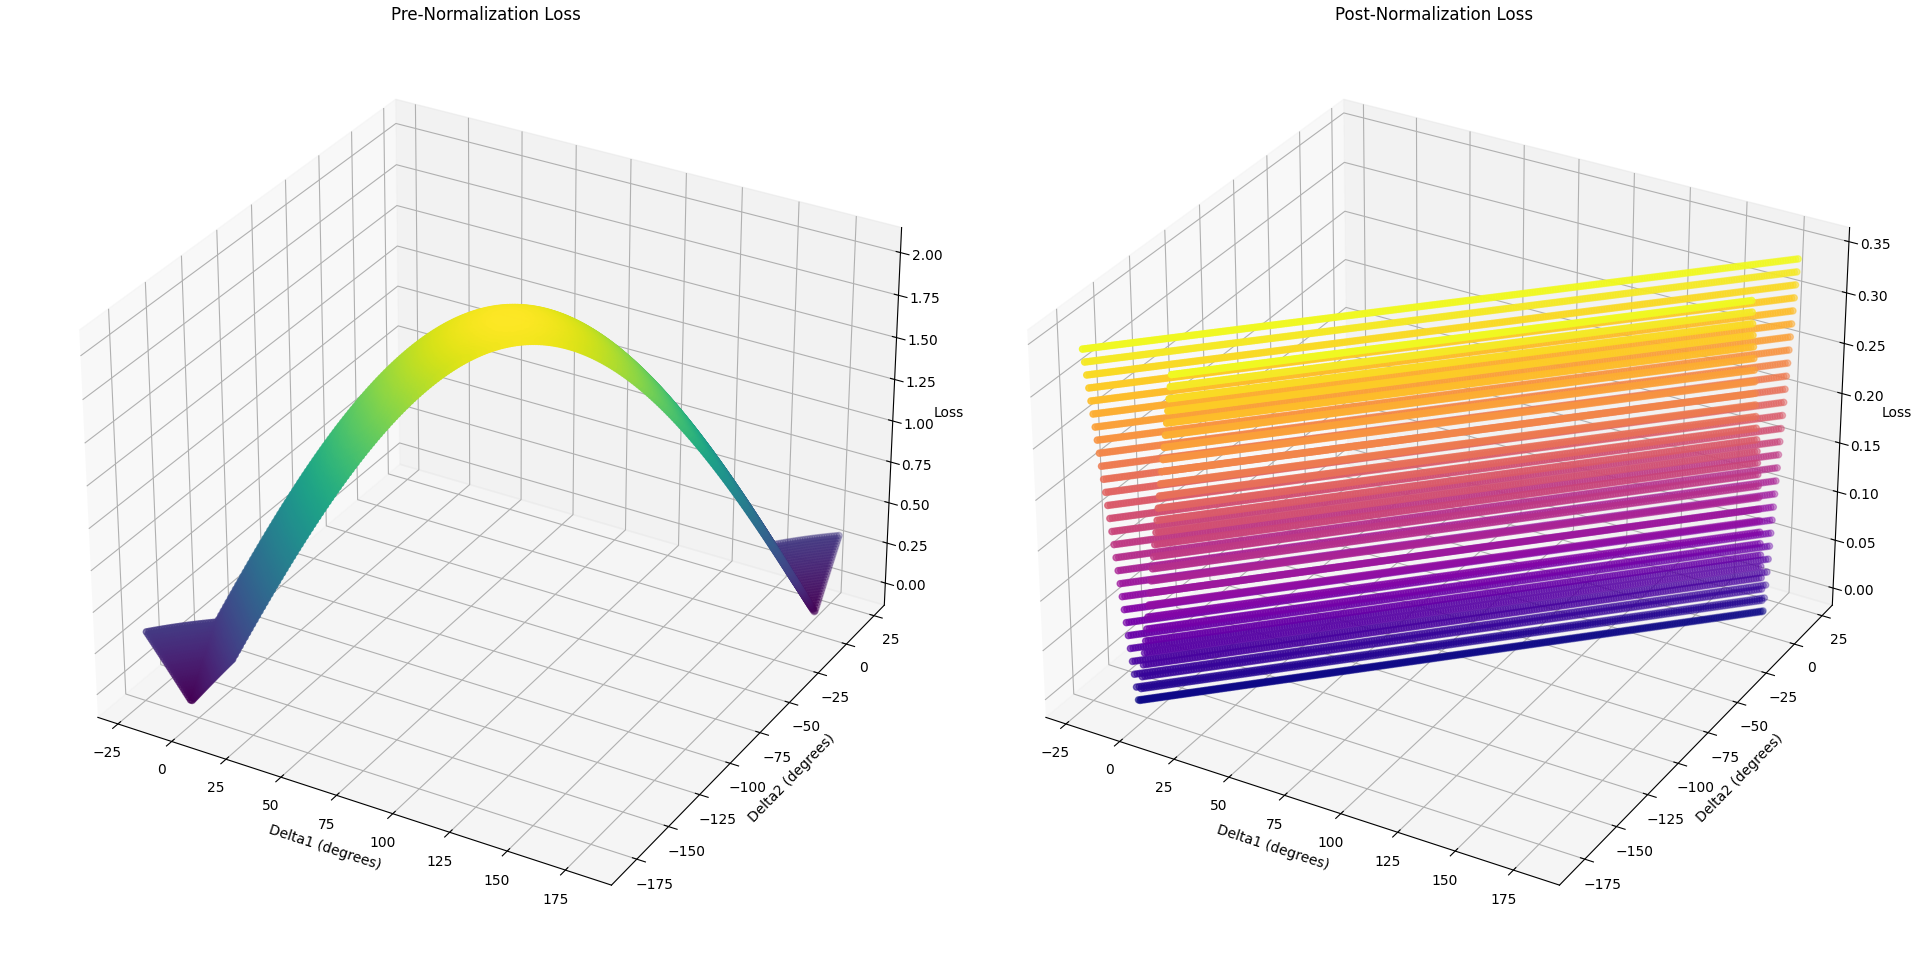
\includegraphics[width=\textwidth]{Chapter 4/Figs4/lossprevspost.png}
    \caption{Loss comparison between pre-normalization and post-normalization methods.}
    \label{fig:lossprevpost}
\end{figure}


As seen in Figure~\ref{fig:lossprevpost}, the pre-normalization method results in losses exceeding 2.0 due to the compounding effect of treating both images independently. In contrast, the post-normalization method, which works with relative rotation, consistently yields lower losses, with a maximum loss of approximately 0.35 under these typical UAV conditions. Further, the losses in the post-normalization method consists of almost all non-mutual information. Therefore, post-normalization is expected to provide more accurate translation estimations due to better retention of keypoint information.


\subsection*{Empirical Validation}

In empirical tests, these results were confirmed, with post-normalization consistently providing higher accuracy due to better retention of keypoint information. The effects were most significant in the DESERT dataset, where the sparsity of keypoints made the dataset particularly sensitive to information loss during rotation. 

\subsection*{Method Conclusion}

Given the UAV's typical flight pattern and the need to minimize information loss, post-normalization is applied. In this approach, images are first aligned, followed by translation estimation. Finally, the translation vector is normalized to the global NE coordinate space for consistent navigation.




\section{Testing Shortlist}

The system design integrates multiple features to ensure robustness, accuracy, and efficiency in UAV navigation tasks. The following components have been selected and tested across various scenarios:

\begin{itemize}
    \item \textbf{Feature Detectors:} AKAZE, SuperPoint (with LightGlue matcher), and ORB. Note, the SuperPoint detector is used in conjunction with the LightGlue matcher to enhance performance.
    \item \textbf{Feature Matchers:} FLANN and BruteForce. KNN 
    \item \textbf{Search Techniques:} KNN with \( K=2 \). Empirical tests showed a value of 1 to be ineffective without Lowe's ratio test, while values above 2 introduced excessive computational overheads. Further, radius search was seen to be unreliable due to the varying density of keypoints across datasets.
    \item \textbf{Transformation Estimation:} Homography, Affine, Partial Affine (Rigid) transformations using OpenCV, and SVD-based rigid transformations for rotation and translation estimations. Rotational and Translational Estimators are tested separately as optimal detectors and parameters may vary for each.
    \item \textbf{Global Image Similarity Measures:} SSIM, histogram matching, local retrofit, and cross-correlation.
    \item \textbf{Optimization Techniques:} Parallel Flow Filtering, LMEDS, RANSAC, Lowe's ratio test, n-Match thresholding, and absolute thresholding for match refinement. Empirical tests indicated that cross-checking was not applicable due to the excessive computational costs involved. KNN
\end{itemize}


\section{Conclusion}

The system design integrates feature extraction, matching, and transformation estimation to enable precise UAV navigation, even in the absence of reliable GPS data. By employing a combination of diverse feature detectors and optimizing various pipeline stages, the system ensures robustness, accuracy, and computational efficiency across different operational scenarios. 

